\subsubsection{Neuroni e feature: una distinzione cruciale}

L'assunzione nascosta è questa: abbiamo implicitamente identificato i \textit{neuroni} con le \textit{feature}. Abbiamo ragionato come se ogni concetto dovesse ``abitare'' in un neurone dedicato, e ogni neurone potesse ospitare un solo concetto. Ma queste due entità—neuroni e feature—sono oggetti profondamente diversi.

\begin{notebox}
\textbf{Neuroni vs Feature}\\
\begin{itemize}
    \item Un \textbf{neurone} (o \textit{dimensione}) è un'unità computazionale della rete: un singolo valore numerico nello spazio delle attivazioni. I neuroni sono gli \textbf{assi} del sistema di coordinate—le direzioni ``cardinali'' lungo cui misuriamo le attivazioni. In BERT-base, ci sono 768 neuroni che definiscono gli assi $d_1, d_2, \dots, d_{768}$.
    
    \item Una \textbf{feature} $f_i$ è un concetto semantico che vorremmo catturare: ``torta al cioccolato'', ``meccanica quantistica'', ``sentimento negativo''. Le feature sono le proprietà \textit{dei dati} che risultano utili per i compiti del modello—i ``fattori generativi'' della semantica.
\end{itemize}
\end{notebox}

La chiave per comprendere la superposition sta nel realizzare che \textit{le feature non devono necessariamente coincidere con gli assi}. Una feature può essere rappresentata come una \textbf{direzione arbitraria} nello spazio—un vettore che punta in una direzione qualsiasi, combinando più neuroni con pesi diversi. Indichiamo con $\mathbf{w}_i \in \mathbb{R}^{768}$ la direzione associata alla feature $f_i$ nello spazio di BERT.

Consideriamo un'analogia geografica, illustrata in Figura~\ref{fig:geographic_analogy}. Se dobbiamo descrivere la posizione di una città, possiamo usare le coordinate cardinali: ``100 km a Nord, 50 km a Est''. Gli assi Nord-Sud ed Est-Ovest sono i nostri ``neuroni''—le direzioni di riferimento del sistema. Ma nulla ci impedisce di descrivere la stessa posizione come ``112 km in direzione Nord-Nord-Est''. La direzione Nord-Nord-Est non coincide con nessun asse, ma è perfettamente definita come combinazione degli assi.

\begin{figure}[htbp]
    \centering
    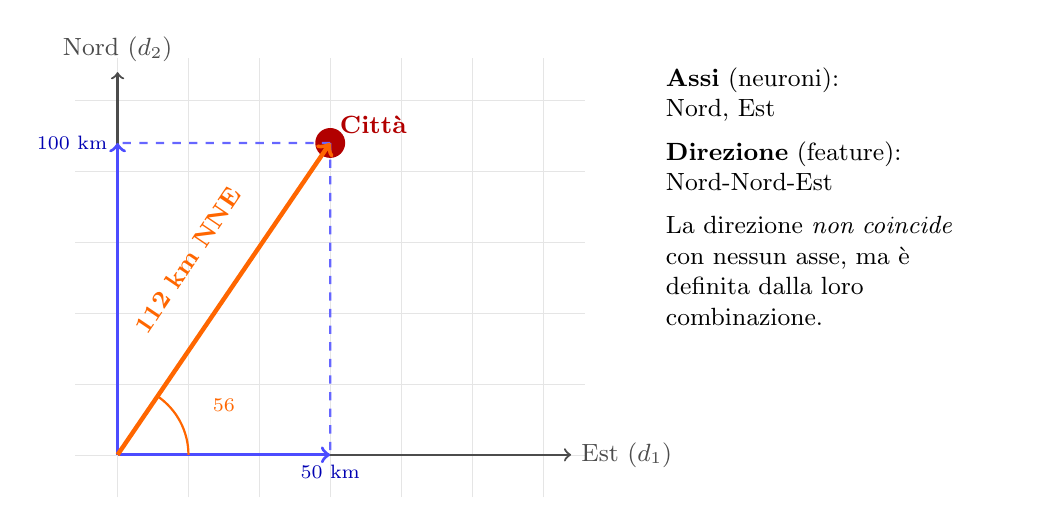
\begin{tikzpicture}[scale=1.8]
        % Griglia di sfondo
        \draw[gray!20, very thin, step=0.5] (-0.3,-0.3) grid (3.3,2.8);
        
        % Assi (neuroni)
        \draw[->, thick, black!70] (0,0) -- (3.2,0) node[right, font=\small] {Est ($d_1$)};
        \draw[->, thick, black!70] (0,0) -- (0,2.7) node[above, font=\small] {Nord ($d_2$)};
        
        % Punto di destinazione
        \coordinate (city) at (1.5, 2.2);
        \fill[red!70!black] (city) circle (3pt);
        \node[anchor=south west, font=\small\bfseries, red!70!black] at (city) {Città};
        
        % Componenti sugli assi (proiezioni tratteggiate)
        \draw[dashed, blue!60, thick] (city) -- (1.5, 0) node[below, font=\scriptsize, blue!70!black] {50 km};
        \draw[dashed, blue!60, thick] (city) -- (0, 2.2) node[left, font=\scriptsize, blue!70!black] {100 km};
        
        % Vettori componenti sugli assi
        \draw[->, very thick, blue!70] (0,0) -- (1.5, 0);
        \draw[->, very thick, blue!70] (0,0) -- (0, 2.2);
        
        % Direzione obliqua (la feature)
        \draw[->, ultra thick, orange!80!red] (0,0) -- (city);
        \node[anchor=south, font=\small\bfseries, orange!80!red, rotate=56] at (0.6, 1.3) {112 km NNE};
        
        % Angolo
        \draw[orange!80!red, thick] (0.5,0) arc (0:56:0.5);
        \node[orange!80!red, font=\scriptsize] at (0.75, 0.35) {$56°$};
        
        % Etichette esplicative
        \node[anchor=north west, font=\small, align=left, text width=4.5cm] at (3.8, 2.8) {
            \textbf{Assi} (neuroni):\\
            Nord, Est\\[0.5em]
            \textbf{Direzione} (feature):\\
            Nord-Nord-Est\\[0.5em]
            La direzione \textit{non coincide}\\
            con nessun asse, ma è\\
            definita dalla loro\\
            combinazione.
        };
    \end{tikzpicture}
    \caption{Analogia geografica tra neuroni e feature. Gli assi cardinali (Nord, Est) rappresentano i neuroni: le direzioni di riferimento del sistema. La direzione Nord-Nord-Est rappresenta una feature: non coincide con nessun asse, ma è definita come loro combinazione ($100 \text{ km Nord} + 50 \text{ km Est} = 112 \text{ km NNE}$). In uno spazio bidimensionale esistono solo 2 assi, ma infinite direzioni.}
    \label{fig:geographic_analogy}
\end{figure}

Allo stesso modo, una feature come $f_{\text{torta}}$ (``torta al cioccolato'') non deve necessariamente corrispondere all'asse $d_{42}$. Può essere rappresentata come una direzione obliqua $\mathbf{w}_{\text{torta}}$ nello spazio delle attivazioni:
\begin{equation}
    \mathbf{w}_{\text{torta}} = 0.7 \cdot \mathbf{d}_1 + 0.5 \cdot \mathbf{d}_2 - 0.3 \cdot \mathbf{d}_3 + \dots
\end{equation}
una combinazione di molti neuroni, nessuno dei quali ``significa'' torta al cioccolato in isolamento.

Questa osservazione apre una possibilità che il ragionamento precedente escludeva: \textit{se le feature sono direzioni e non assi, possiamo avere più feature che neuroni}. In uno spazio tridimensionale esistono solo tre assi, ma infinite direzioni. La domanda diventa: quante direzioni ``utili'' possiamo stipare in uno spazio a $n$ dimensioni?
\subsubsection{La geometria della superposition}

Torniamo al nostro esempio con neuroni e feature, ma questa volta ragioniamo geometricamente. Consideriamo uno spazio semplificato con soli due neuroni—due assi, $d_1$ e $d_2$—e vediamo cosa succede al variare del numero di feature da rappresentare.

\paragraph{Caso ideale: due feature, due neuroni.}
Supponiamo di avere esattamente due feature da rappresentare: $f_{\text{torta}}$ (``torta al cioccolato'') e $f_{\text{quant}}$ (``meccanica quantistica''). Con due neuroni a disposizione, possiamo assegnare a ciascuna feature un asse dedicato. Le direzioni $\mathbf{w}_{\text{torta}}$ e $\mathbf{w}_{\text{quant}}$ coincidono con gli assi:

\begin{equation}
    \mathbf{w}_{\text{torta}} = \begin{pmatrix} 1 \\ 0 \end{pmatrix} = \mathbf{d}_1, \qquad
    \mathbf{w}_{\text{quant}} = \begin{pmatrix} 0 \\ 1 \end{pmatrix} = \mathbf{d}_2
\end{equation}

Questa è una rappresentazione perfettamente \textit{disentangled}: ogni feature coincide con un asse. Le due direzioni sono \textbf{ortogonali}—il loro prodotto scalare è zero ($\mathbf{w}_{\text{torta}} \cdot \mathbf{w}_{\text{quant}} = 0$)—il che significa che sono completamente indipendenti.

In questa configurazione, l'embedding $\mathbf{x}$ di un input si scrive come semplice combinazione:
\begin{equation}
    \mathbf{x} = a_{\text{torta}} \cdot \mathbf{w}_{\text{torta}} + a_{\text{quant}} \cdot \mathbf{w}_{\text{quant}} = \begin{pmatrix} a_{\text{torta}} \\ a_{\text{quant}} \end{pmatrix}
\end{equation}
dove $a_{\text{torta}}$ e $a_{\text{quant}}$ sono le \textit{intensità} con cui ogni feature è presente nell'input (zero se la feature è assente, positiva se presente).

Interpretare $\mathbf{x}$ è banale: la prima coordinata ci dice direttamente quanto è attiva la feature $f_{\text{torta}}$, la seconda quanto è attiva $f_{\text{quant}}$. Nessuna ambiguità, nessuna interferenza. Questo è il mondo ideale in cui vorremmo vivere.

\begin{figure}[htbp]
    \centering
    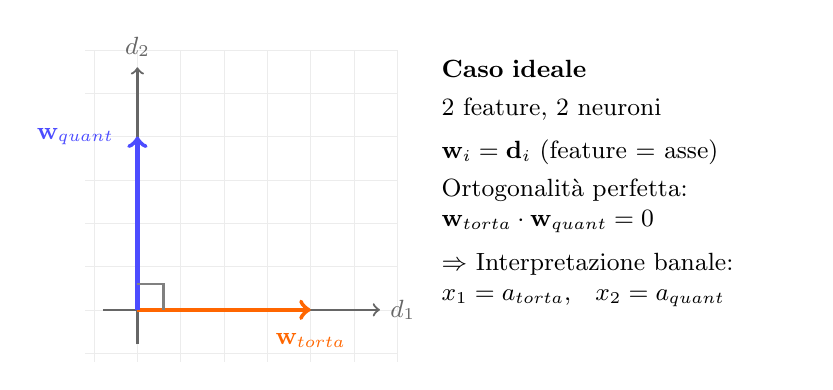
\begin{tikzpicture}[scale=2.2]
        % Griglia
        \draw[gray!15, very thin, step=0.25] (-0.3,-0.3) grid (1.5,1.5);
        
        % Assi (neuroni)
        \draw[->, thick, black!60] (-0.2,0) -- (1.4,0) node[right, font=\small] {$d_1$};
        \draw[->, thick, black!60] (0,-0.2) -- (0,1.4) node[above, font=\small] {$d_2$};
        
        % Feature allineate agli assi
        \draw[->, ultra thick, orange!80!red] (0,0) -- (1,0);
        \node[anchor=north, font=\small\bfseries, orange!80!red] at (1, -0.08) {$\mathbf{w}_{\text{torta}}$};
        
        \draw[->, ultra thick, blue!70] (0,0) -- (0,1);
        \node[anchor=east, font=\small\bfseries, blue!70] at (-0.08, 1) {$\mathbf{w}_{\text{quant}}$};
        
        % Angolo retto
        \draw[thick, black!50] (0.15,0) -- (0.15,0.15) -- (0,0.15);
        
        % Etichetta
        \node[anchor=north west, font=\small, align=left, text width=4.5cm] at (1.7, 1.5) {
            \textbf{Caso ideale}\\[0.3em]
            2 feature, 2 neuroni\\[0.5em]
            $\mathbf{w}_i = \mathbf{d}_i$ (feature $=$ asse)\\[0.3em]
            Ortogonalità perfetta:\\
            $\mathbf{w}_{\text{torta}} \cdot \mathbf{w}_{\text{quant}} = 0$\\[0.5em]
            $\Rightarrow$ Interpretazione banale:\\
            $x_1 = a_{\text{torta}}$, \; $x_2 = a_{\text{quant}}$
        };
    \end{tikzpicture}
    \caption{Rappresentazione disentangled ideale. Con due feature e due neuroni, ogni direzione $\mathbf{w}_i$ coincide con un asse $\mathbf{d}_i$. Le coordinate di $\mathbf{x}$ indicano direttamente le intensità $a_i$ di ciascuna feature.}
    \label{fig:ideal_two_features}
\end{figure}

\paragraph{Il problema: tre feature, due neuroni.}
Aggiungiamo ora una terza feature: $f_{\text{ricetta}}$ (``ricetta di cucina''). Improvvisamente ci troviamo in difficoltà: lo spazio ha solo due assi, ma tre feature da rappresentare. Nella logica del mondo ideale, dovremmo rinunciare a una delle tre—non c'è spazio per tutte sugli assi.
Ma esiste un'alternativa. Se accettiamo che le direzioni $\mathbf{w}_i$ non debbano coincidere con gli assi, possiamo rappresentare tutte e tre le feature come \textit{direzioni} nel piano. La configurazione geometricamente ottimale è quella che le rende il più possibile ``separate''—il più possibile ortogonali, nei limiti del vincolo dimensionale.
In due dimensioni, la migliore disposizione per tre vettori unitari è quella che li distribuisce uniformemente: tre direzioni a 120° l'una dall'altra, come i vertici di un triangolo equilatero centrato nell'origine.

\begin{figure}[htbp]
    \centering
    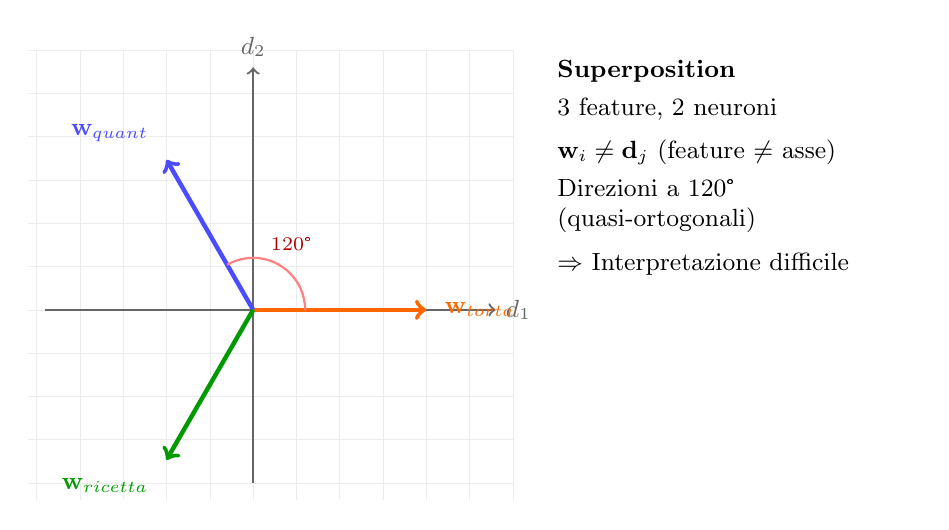
\begin{tikzpicture}[scale=2.2]
        % Griglia
        \draw[gray!15, very thin, step=0.25] (-1.3,-1.1) grid (1.5,1.5);
        
        % Assi (neuroni)
        \draw[->, thick, black!60] (-1.2,0) -- (1.4,0) node[right, font=\small] {$d_1$};
        \draw[->, thick, black!60] (0,-1.0) -- (0,1.4) node[above, font=\small] {$d_2$};
        
        % Tre feature a 120° (direzioni quasi-ortogonali)
        % w_torta: 0°
        \draw[->, ultra thick, orange!80!red] (0,0) -- (1,0);
        \node[anchor=west, font=\small\bfseries, orange!80!red] at (1.05, 0) {$\mathbf{w}_{\text{torta}}$};
        
        % w_quant: 120°
        \draw[->, ultra thick, blue!70] (0,0) -- ({cos(120)},{sin(120)});
        \node[anchor=south east, font=\small\bfseries, blue!70] at ({cos(120)-0.05},{sin(120)+0.05}) {$\mathbf{w}_{\text{quant}}$};
        
        % w_ricetta: 240°
        \draw[->, ultra thick, green!60!black] (0,0) -- ({cos(240)},{sin(240)});
        \node[anchor=north east, font=\small\bfseries, green!60!black] at ({cos(240)-0.05},{sin(240)-0.05}) {$\mathbf{w}_{\text{ricetta}}$};
        
        % Angoli
        \draw[red!50, thick] (0.3,0) arc (0:120:0.3);
        \node[red!70!black, font=\scriptsize] at (0.22, 0.38) {120°};
        
        % Etichetta
        \node[anchor=north west, font=\small, align=left, text width=4.5cm] at (1.7, 1.5) {
            \textbf{Superposition}\\[0.3em]
            3 feature, 2 neuroni\\[0.5em]
            $\mathbf{w}_i \neq \mathbf{d}_j$ (feature $\neq$ asse)\\[0.3em]
            Direzioni a 120°\\
            (quasi-ortogonali)\\[0.5em]
            $\Rightarrow$ Interpretazione difficile
        };
    \end{tikzpicture}
    \caption{Superposition: tre feature in due dimensioni. Le direzioni $\mathbf{w}_i$ non coincidono più con gli assi; sono disposte a 120° l'una dall'altra—la configurazione che massimizza la ``separazione'' nel piano.}
    \label{fig:superposition_three_features}
\end{figure}
Questa configurazione è ciò che Elhage et al.~\parencite{elhage2022superposition} chiamano \textbf{superposition}: la rete rappresenta più feature di quanti siano i neuroni disponibili, codificando le direzioni $\mathbf{w}_i$ come vettori quasi-ortogonali nello spazio delle attivazioni.
\begin{notebox}
\textbf{Superposition Hypothesis}\\
Le reti neurali rappresentano $m$ feature in uno spazio di $n$ dimensioni, con $m > n$, codificando ogni feature $f_i$ come una \textbf{direzione} (vettore unitario) $\mathbf{w}_i$ nello spazio delle attivazioni. Le direzioni sono scelte per essere il più possibile \textit{quasi-ortogonali}—indipendenti nei limiti del vincolo dimensionale. Il risultato è una rappresentazione compressa ma \textit{polisemantica}: ogni neurone partecipa alla codifica di molteplici feature.
\end{notebox}

\paragraph{Il principio di sovrapposizione lineare.}
Anche in superposition, l'embedding $\mathbf{x}$ di un input si scrive come combinazione delle direzioni delle feature attive:
\begin{equation}
    \mathbf{x} = \sum_{i} a_i \, \mathbf{w}_i = a_{\text{torta}} \, \mathbf{w}_{\text{torta}} + a_{\text{quant}} \, \mathbf{w}_{\text{quant}} + a_{\text{ricetta}} \, \mathbf{w}_{\text{ricetta}} + \dots
    \label{eq:linear_superposition}
\end{equation}
dove $a_i \geq 0$ è l'intensità della feature $f_i$ (zero se assente). Questo è il \textbf{principio di sovrapposizione} dei sistemi lineari: la risposta a stimoli combinati è la somma delle risposte ai singoli stimoli.
\begin{notebox}
\textbf{Principio di Sovrapposizione}\\
Per un sistema lineare, la risposta a una combinazione di input è la combinazione delle risposte individuali. Se l'input $A$ produce la risposta $X$, e l'input $B$ produce la risposta $Y$, allora l'input $(A + B)$ produce la risposta $(X + Y)$.
Formalmente, una funzione $F$ soddisfa il principio di sovrapposizione se e solo se è \textit{lineare}:
\begin{align}
    F(x_1 + x_2) &= F(x_1) + F(x_2) && \text{(additività)} \\
    F(\alpha x) &= \alpha F(x) && \text{(omogeneità)}
\end{align}
\end{notebox}

\paragraph{L'opacità: direzioni sconosciute.}
L'equazione~\eqref{eq:linear_superposition} ci dice che l'embedding $\mathbf{x}$ è una combinazione delle direzioni $\mathbf{w}_i$ con intensità $a_i$. In linea di principio, \textit{se conoscessimo} le direzioni, potremmo tentare di recuperare le intensità.
Ma nella pratica:
\begin{itemize}
    \item \textbf{Osserviamo} solo $\mathbf{x}$—il vettore risultante, l'embedding prodotto da BERT
    \item \textbf{Non conosciamo} le direzioni $\mathbf{w}_i$—la rete le ha apprese durante l'addestramento, ma non ce le rivela
    \item \textbf{Non conosciamo} le intensità $a_i$—non sappiamo quali feature $f_i$ sono attive né con quale forza
\end{itemize}
Questa è l'\textbf{opacità} delle rappresentazioni neurali: l'informazione semantica è codificata in $\mathbf{x}$, ma non possiamo estrarla perché non conosciamo la ``chiave di decodifica''—le direzioni $\mathbf{w}_i$ delle feature.
Ma anche se, per magia, conoscessimo le direzioni, rimarrebbe un secondo problema: nella superposition, le direzioni non sono ortogonali. E questo causa interferenza.


\subsubsection{Il problema dell'interferenza}

Supponiamo, per un momento, di conoscere le direzioni $\mathbf{w}_i$. Potremmo allora tentare di recuperare le intensità $a_i$ dall'embedding osservato $\mathbf{x}$? La risposta è: solo approssimativamente, e con un errore sistematico.

\paragraph{Decodifica nel caso ideale.}
Nel caso disentangled (Figura~\ref{fig:ideal_two_features}), le direzioni coincidono con gli assi e sono perfettamente ortogonali. Se vogliamo sapere quanto è attiva la feature $f_{\text{torta}}$, calcoliamo il prodotto scalare tra $\mathbf{x}$ e la direzione $\mathbf{w}_{\text{torta}}$:
\begin{equation}
    \mathbf{x} \cdot \mathbf{w}_{\text{torta}} = \left( a_{\text{torta}} \, \mathbf{w}_{\text{torta}} + a_{\text{quant}} \, \mathbf{w}_{\text{quant}} \right) \cdot \mathbf{w}_{\text{torta}}
\end{equation}

Poiché $\mathbf{w}_{\text{torta}} \cdot \mathbf{w}_{\text{torta}} = 1$ (vettore unitario) e $\mathbf{w}_{\text{quant}} \cdot \mathbf{w}_{\text{torta}} = 0$ (ortogonalità), otteniamo:
\begin{equation}
    \mathbf{x} \cdot \mathbf{w}_{\text{torta}} = a_{\text{torta}} \cdot 1 + a_{\text{quant}} \cdot 0 = a_{\text{torta}}
\end{equation}

Perfetto: il prodotto scalare restituisce esattamente l'intensità cercata, senza contaminazioni. L'ortogonalità garantisce che le feature non si ``vedano'' a vicenda.

\paragraph{Decodifica in superposition: l'interferenza.}
Nel caso della superposition (Figura~\ref{fig:superposition_three_features}), le direzioni non sono ortogonali. Calcoliamo i prodotti scalari tra le nostre tre direzioni a 120°:

\begin{equation}
    \mathbf{w}_{\text{torta}} = \begin{pmatrix} 1 \\ 0 \end{pmatrix}, \quad
    \mathbf{w}_{\text{quant}} = \begin{pmatrix} -0.5 \\ 0.866 \end{pmatrix}, \quad
    \mathbf{w}_{\text{ricetta}} = \begin{pmatrix} -0.5 \\ -0.866 \end{pmatrix}
\end{equation}

I prodotti scalari tra coppie di direzioni sono:
\begin{equation}
    \mathbf{w}_{\text{torta}} \cdot \mathbf{w}_{\text{quant}} = 1 \cdot (-0.5) + 0 \cdot 0.866 = -0.5 \neq 0
\end{equation}
Le direzioni non sono ortogonali—hanno una ``sovrapposizione'' non nulla. Cosa comporta questo in pratica?
\paragraph{Esempio: interferenza concreta.}
Consideriamo un input che riguarda \textit{solo} torte al cioccolato: la feature $f_{\text{torta}}$ è attiva con intensità $a_{\text{torta}} = 1$, mentre le altre sono inattive ($a_{\text{quant}} = a_{\text{ricetta}} = 0$). L'embedding risultante è semplicemente:
\begin{equation}
    \mathbf{x} = 1 \cdot \mathbf{w}_{\text{torta}} + 0 \cdot \mathbf{w}_{\text{quant}} + 0 \cdot \mathbf{w}_{\text{ricetta}} = \begin{pmatrix} 1 \\ 0 \end{pmatrix}
\end{equation}
Ora proviamo a ``decodificare'' quanto sembra attiva la feature $f_{\text{quant}}$:
\begin{equation}
    \mathbf{x} \cdot \mathbf{w}_{\text{quant}} = \begin{pmatrix} 1 \\ 0 \end{pmatrix} \cdot \begin{pmatrix} -0.5 \\ 0.866 \end{pmatrix} = -0.5
\end{equation}
Il risultato è $-0.5$, non zero! Nonostante la feature ``meccanica quantistica'' sia completamente assente dall'input, il prodotto scalare restituisce un valore non nullo. Questo è il \textbf{rumore di interferenza}: la non-ortogonalità delle direzioni causa un ``leakage'' tra feature. Quando una feature si attiva, altre feature non correlate mostrano attivazioni spurie.
\begin{figure}[htbp]
    \centering
    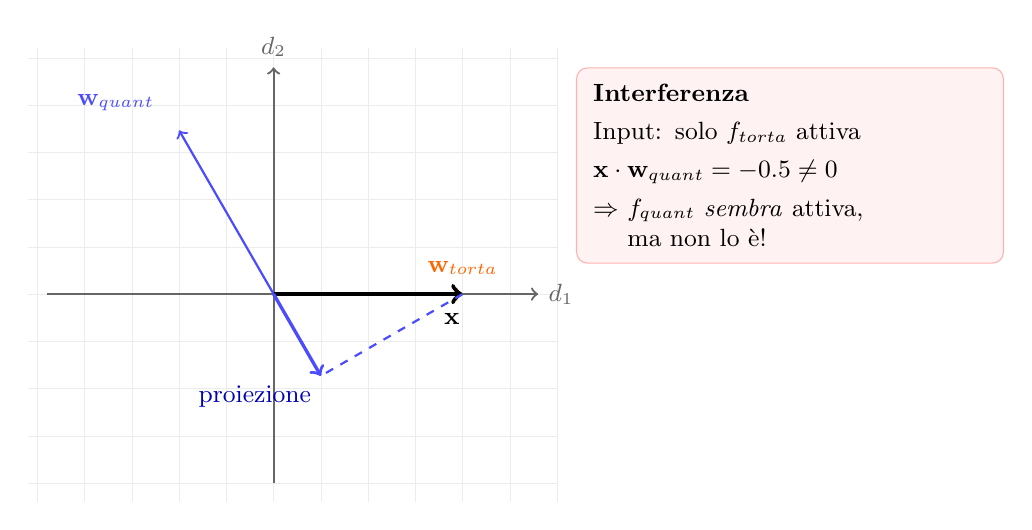
\begin{tikzpicture}[scale=2.4]
        % Griglia
        \draw[gray!15, very thin, step=0.25] (-1.3,-1.1) grid (1.5,1.3);
        
        % Assi (neuroni)
        \draw[->, thick, black!60] (-1.2,0) -- (1.4,0) node[right, font=\small] {$d_1$};
        \draw[->, thick, black!60] (0,-1.0) -- (0,1.2) node[above, font=\small] {$d_2$};
        
        % Direzioni delle feature
        \draw[->, thick, orange!80!red] (0,0) -- (1,0);
        \node[anchor=south, font=\small\bfseries, orange!80!red] at (1, 0.05) {$\mathbf{w}_{\text{torta}}$};
        
        \draw[->, thick, blue!70] (0,0) -- ({cos(120)},{sin(120)});
        \node[anchor=south east, font=\small\bfseries, blue!70] at ({cos(120)-0.08},{sin(120)+0.05}) {$\mathbf{w}_{\text{quant}}$};
        
        % Vettore x osservato (solo torta attiva)
        \draw[->, ultra thick, black] (0,0) -- (1,0);
        \node[anchor=north west, font=\small] at (0.85, -0.05) {$\mathbf{x}$};
        
        % Proiezione di x su w_quant
        \coordinate (proj) at ({cos(120)*(-0.5)},{sin(120)*(-0.5)});
        \draw[dashed, blue!70, thick] (1,0) -- (proj);
        \draw[->, blue!70, very thick] (0,0) -- (proj);
        \node[blue!70!black, font=\small, anchor=north east] at (proj) {proiezione};
        
        % Etichetta interferenza
        \node[anchor=north west, font=\small, align=left, text width=5cm, fill=red!5, draw=red!30, rounded corners, inner sep=6pt] at (1.6, 1.2) {
            \textbf{Interferenza}\\[0.3em]
            Input: solo $f_{\text{torta}}$ attiva\\[0.3em]
            $\mathbf{x} \cdot \mathbf{w}_{\text{quant}} = -0.5 \neq 0$\\[0.3em]
            $\Rightarrow$ $f_{\text{quant}}$ \textit{sembra} attiva,\\
            \phantom{$\Rightarrow$} ma non lo è!
        };
    \end{tikzpicture}
    \caption{Interferenza nella superposition. L'input contiene solo ``torta al cioccolato'' ($\mathbf{x} = \mathbf{w}_{\text{torta}}$), ma la proiezione su $\mathbf{w}_{\text{quant}}$ è non nulla ($-0.5$). La non-ortogonalità causa attivazioni spurie: feature inattive sembrano parzialmente attive.}
    \label{fig:interference}
\end{figure}

\paragraph{Il costo della compressione.}
L'interferenza è il prezzo da pagare per la superposition. Abbiamo guadagnato la possibilità di rappresentare più feature che neuroni, ma abbiamo perso la separabilità perfetta. Ogni volta che ``leggiamo'' l'attivazione di una feature, il segnale è contaminato dalle altre.
In formule, se proviamo a decodificare l'intensità $a_i$ tramite il prodotto scalare:
\begin{equation}
    \mathbf{x} \cdot \mathbf{w}_i = \sum_j a_j \, (\mathbf{w}_j \cdot \mathbf{w}_i) = a_i + \sum_{j \neq i} a_j \, (\mathbf{w}_j \cdot \mathbf{w}_i)
    \label{eq:interference}
\end{equation}
Il primo termine è il segnale che cerchiamo ($a_i$). Il secondo termine è il rumore di interferenza—la somma dei contributi di tutte le altre feature, pesati per quanto le loro direzioni sono ``allineate'' con $\mathbf{w}_i$. Solo se tutte le direzioni fossero ortogonali ($\mathbf{w}_j \cdot \mathbf{w}_i = 0$ per $j \neq i$), il rumore svanirebbe.
A questo punto la superposition sembra un pessimo affare: comprimiamo le feature, ma le rendiamo inseparabili. Perché mai una rete neurale dovrebbe adottare questa strategia?

\subsubsection{Perché funziona comunque: la sparsità delle feature}

L'interferenza sembra un problema grave: se ogni volta che decodifichiamo una feature otteniamo un segnale contaminato dalle altre, come può la rete funzionare correttamente? La risposta sta in un'osservazione empirica cruciale: \textbf{le feature sono sparse}.

\paragraph{Feature sparse nel mondo reale.}
Consideriamo i concetti che un modello linguistico deve rappresentare. ``Meccanica quantistica'' è rilevante solo in una minuscola frazione dei testi—articoli scientifici, manuali di fisica, discussioni specialistiche. ``Torta al cioccolato'' compare in contesti completamente diversi—ricette, blog culinari, menu di ristoranti. ``Legislazione fiscale'', ``errore di sintassi'', ``partita di calcio''—ciascun concetto ha il suo dominio ristretto.
In un dato input, solo \textit{pochi} concetti tra le migliaia possibili sono effettivamente pertinenti. Una frase sul calcio non menziona la meccanica quantistica; una ricetta di dolci non discute di legislazione fiscale. Le feature sono \textbf{sparse}: la maggior parte ha intensità $a_i = 0$ per la maggior parte degli input.
\paragraph{Sparsità e interferenza.}
Torniamo all'equazione dell'interferenza~\eqref{eq:interference}:
\begin{equation*}
    \mathbf{x} \cdot \mathbf{w}_i = a_i + \sum_{j \neq i} a_j \, (\mathbf{w}_j \cdot \mathbf{w}_i)
\end{equation*}
Il rumore di interferenza dipende dai prodotti $a_j \cdot (\mathbf{w}_j \cdot \mathbf{w}_i)$. Ma se la feature $f_j$ è inattiva ($a_j = 0$), il suo contributo al rumore è nullo—indipendentemente da quanto $\mathbf{w}_j$ sia allineata con $\mathbf{w}_i$.
Questo significa che \textit{l'interferenza si manifesta solo tra feature simultaneamente attive}. Se $f_{\text{torta}}$ e $f_{\text{quant}}$ non sono mai attive nello stesso input, possono condividere direzioni parzialmente sovrapposte senza mai interferire in pratica.
\begin{notebox}
\textbf{Sparsità e Superposition}\\
La superposition è vantaggiosa quando le feature sono sparse. Se ogni input attiva solo una piccola frazione delle feature totali, l'interferenza potenziale (dovuta alla non-ortogonalità) raramente si manifesta in pratica. La rete può ``stipare'' molte più feature di quanti siano i neuroni, accettando un piccolo rischio di interferenza nei rari casi di co-occorrenza.
\end{notebox}

\paragraph{Il trade-off sparsità-capacità.}
Emerge quindi un trade-off fondamentale, illustrato in Figura~\ref{fig:sparsity_superposition}. Al crescere della sparsità delle feature, la rete può permettersi di rappresentarne sempre di più nello stesso spazio:

\begin{enumerate}
    \item Sparsità 0\% (ogni feature sempre attiva): l'unica rappresentazione senza interferenza è quella disentangled—ogni feature su un asse dedicato. Se abbiamo $n$ neuroni, possiamo rappresentare al massimo $n$ feature.    
    \item Sparsità moderata (es. 50\%): le feature si attivano metà delle volte. Possiamo iniziare a usare direzioni non allineate agli assi, accettando interferenza occasionale. La capacità cresce oltre $n$.
    \item Sparsità alta (es. 90\%): le feature si attivano raramente. Possiamo ``stipare'' molte più feature come direzioni quasi-ortogonali—l'interferenza è rara perché le co-occorrenze sono rare. La capacità può crescere significativamente oltre $n$.
\end{enumerate}

\begin{figure}[htbp]
    \centering
    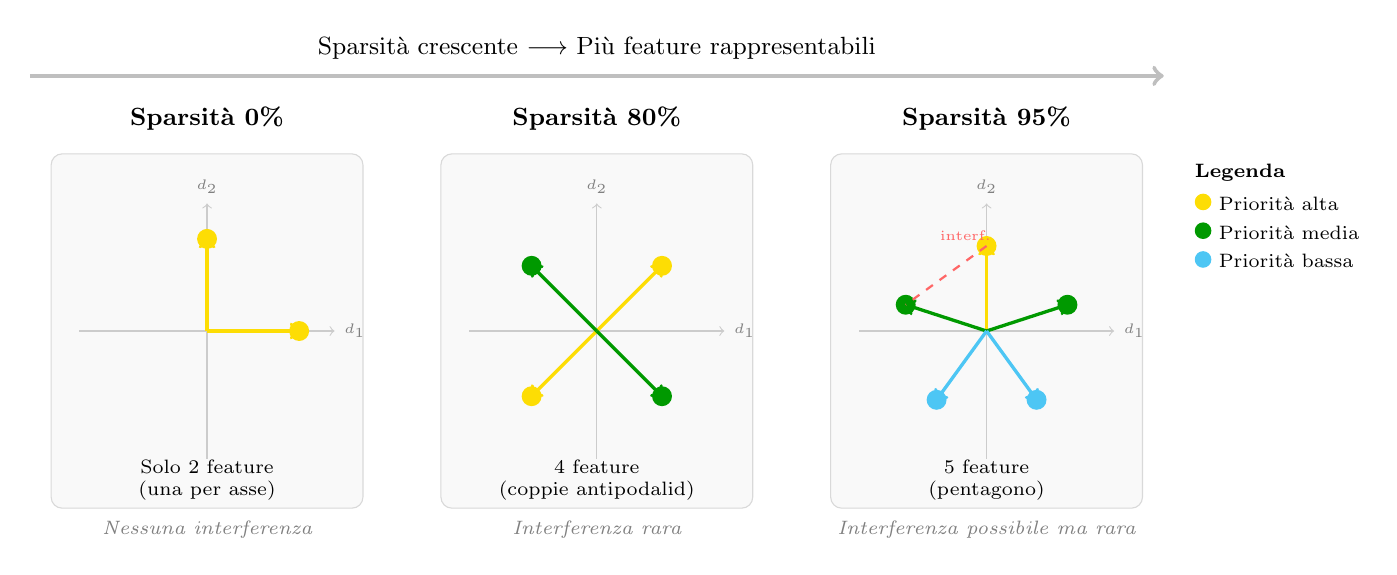
\begin{tikzpicture}[scale=0.9]    
        % === BOX 1: Sparsità 0% ===
        \draw[rounded corners, fill=gray!5, draw=gray!30] (-2.2,-2.5) rectangle (2.2,2.5);
        \node[font=\small\bfseries] at (0, 3) {Sparsità 0\%};     
        % Assi
        \draw[->, gray!40] (-1.8, 0) -- (1.8, 0) node[right, font=\tiny, gray] {$d_1$};
        \draw[->, gray!40] (0, -1.8) -- (0, 1.8) node[above, font=\tiny, gray] {$d_2$};
        % 2 feature sugli assi (ortogonali)
        \draw[->, very thick, yellow!80!orange] (0,0) -- (1.3,0);
        \draw[->, very thick, yellow!80!orange] (0,0) -- (0,1.3);
        \fill[yellow!80!orange] (1.3,0) circle (4pt);
        \fill[yellow!80!orange] (0,1.3) circle (4pt);
        \node[font=\scriptsize, align=center, text width=2.5cm] at (0, -2.1) {
            Solo 2 feature\\(una per asse)
        };
        \node[font=\scriptsize\itshape, gray] at (0, -2.8) {Nessuna interferenza};
        % === BOX 2: Sparsità 80% ===
        \begin{scope}[shift={(5.5,0)}]
            \draw[rounded corners, fill=gray!5, draw=gray!30] (-2.2,-2.5) rectangle (2.2,2.5);
            \node[font=\small\bfseries] at (0, 3) {Sparsità 80\%};
            % Assi
            \draw[->, gray!40] (-1.8, 0) -- (1.8, 0) node[right, font=\tiny, gray] {$d_1$};
            \draw[->, gray!40] (0, -1.8) -- (0, 1.8) node[above, font=\tiny, gray] {$d_2$};
            % 4 feature: due coppie antipodalid su assi obliqui
            % Coppia 1: asse a 45° (giallo)
            \draw[->, very thick, yellow!80!orange] (0,0) -- (0.92, 0.92);
            \draw[->, very thick, yellow!80!orange] (0,0) -- (-0.92, -0.92);
            \fill[yellow!80!orange] (0.92, 0.92) circle (4pt);
            \fill[yellow!80!orange] (-0.92, -0.92) circle (4pt);
            % Coppia 2: asse a -45° (verde)
            \draw[->, very thick, green!60!black] (0,0) -- (0.92, -0.92);
            \draw[->, very thick, green!60!black] (0,0) -- (-0.92, 0.92);
            \fill[green!60!black] (0.92, -0.92) circle (4pt);
            \fill[green!60!black] (-0.92, 0.92) circle (4pt);
            \node[font=\scriptsize, align=center, text width=2.8cm] at (0, -2.1) {
                4 feature\\(coppie antipodalid)
            };
            \node[font=\scriptsize\itshape, gray] at (0, -2.8) {Interferenza rara};
        \end{scope}
        % === BOX 3: Sparsità 95% ===
        \begin{scope}[shift={(11,0)}]
            \draw[rounded corners, fill=gray!5, draw=gray!30] (-2.2,-2.5) rectangle (2.2,2.5);
            \node[font=\small\bfseries] at (0, 3) {Sparsità 95\%};
            % Assi
            \draw[->, gray!40] (-1.8, 0) -- (1.8, 0) node[right, font=\tiny, gray] {$d_1$};
            \draw[->, gray!40] (0, -1.8) -- (0, 1.8) node[above, font=\tiny, gray] {$d_2$};
            % 5 feature come pentagono (72° tra loro)
            \draw[->, very thick, yellow!80!orange] (0,0) -- ({1.2*cos(90)}, {1.2*sin(90)});
            \fill[yellow!80!orange] ({1.2*cos(90)}, {1.2*sin(90)}) circle (4pt);
            \draw[->, very thick, green!60!black] (0,0) -- ({1.2*cos(162)}, {1.2*sin(162)});
            \fill[green!60!black] ({1.2*cos(162)}, {1.2*sin(162)}) circle (4pt);
            \draw[->, very thick, green!60!black] (0,0) -- ({1.2*cos(18)}, {1.2*sin(18)});
            \fill[green!60!black] ({1.2*cos(18)}, {1.2*sin(18)}) circle (4pt);
        
            \draw[->, very thick, cyan!70] (0,0) -- ({1.2*cos(234)}, {1.2*sin(234)});
            \fill[cyan!70] ({1.2*cos(234)}, {1.2*sin(234)}) circle (4pt);
            
            \draw[->, very thick, cyan!70] (0,0) -- ({1.2*cos(306)}, {1.2*sin(306)});
            \fill[cyan!70] ({1.2*cos(306)}, {1.2*sin(306)}) circle (4pt);
            
            % Linea di interferenza tra feature vicine
            \draw[dashed, red!60, thick] ({1.2*cos(90)}, {1.2*sin(90)}) -- ({1.2*cos(162)}, {1.2*sin(162)});
            \node[red!60, font=\tiny] at (-0.3, 1.35) {interf.};
            
            \node[font=\scriptsize, align=center, text width=2.8cm] at (0, -2.1) {
                5 feature\\(pentagono)
            };
            \node[font=\scriptsize\itshape, gray] at (0, -2.8) {Interferenza possibile ma rara};
        \end{scope}
        
        % Freccia sparsità crescente
        \draw[->, ultra thick, gray!50] (-2.5, 3.6) -- (13.5, 3.6);
        \node[font=\small, above] at (5.5, 3.7) {Sparsità crescente $\longrightarrow$ Più feature rappresentabili};
        
        % Legenda
        \node[anchor=north west, font=\scriptsize, align=left] at (13.8, 2.5) {
            \textbf{Legenda}\\[0.5em]
            \tikz\fill[yellow!80!orange] (0,0) circle (3pt); Priorità alta\\[0.3em]
            \tikz\fill[green!60!black] (0,0) circle (3pt); Priorità media\\[0.3em]
            \tikz\fill[cyan!70] (0,0) circle (3pt); Priorità bassa
        };
    \end{tikzpicture}
    \caption{Superposition al variare della sparsità (adattato da Elhage et al.~\parencite{elhage2022superposition}). Con sparsità 0\%, solo 2 feature ottengono assi dedicati (ortogonali). Con sparsità 80\%, 4 feature vengono rappresentate come coppie antipodalid su due assi obliqui (a 45° e -45°). Con sparsità 95\%, 5 feature sono distribuite come un pentagono—l'interferenza tra direzioni vicine è possibile, ma rara grazie alla bassa probabilità di co-occorrenza.}
    \label{fig:sparsity_superposition}
\end{figure}

\paragraph{La strategia ottimale della rete.}
Perché le reti neurali adottano la superposition? Perché è \textit{conveniente}. Il mondo del linguaggio naturale è dominato da feature sparse: la maggior parte dei concetti è rilevante solo in contesti specifici. In questa situazione, dedicare un neurone intero a ogni concetto sarebbe uno spreco—quel neurone resterebbe inattivo per la stragrande maggioranza degli input.
La superposition permette di sfruttare la capacità della rete in modo più efficiente: ``ricicla'' gli stessi neuroni per feature diverse, confidando nel fatto che raramente serviranno contemporaneamente. È una forma di \textbf{compressione lossy}—perdiamo la perfetta separabilità, ma guadagniamo enormemente in capacità rappresentativa.
Questo spiega come BERT possa rappresentare decine di migliaia di concetti con soli 768 neuroni: le feature sono codificate come direzioni quasi-ortogonali, e la sparsità naturale del linguaggio garantisce che l'interferenza, pur possibile in linea di principio, sia rara in pratica.

%https://claude.ai/chat/a893ee36-8c08-401b-b4be-f02cb99770a5